\documentclass[a4paper,12pt]{article}
\usepackage[top=1cm, bottom=2cm, left=2cm, right=2cm]{geometry}
\usepackage{graphicx} % Required for inserting images
\usepackage{amsmath}  % Required for mathematical formulas
\usepackage{amssymb}  % Required for math symbols
\usepackage{float}     % Required for placing figures
\usepackage{longtable} % Required for long tables
\usepackage{hyperref} % Required for adding links and customizing them
\usepackage{booktabs}
\usepackage{ctex}
\usepackage{caption}
\usepackage{tikz}
\usepackage{svg}
% Define custom options for the document class: "student" and "teacher"
\usepackage{enumitem} % For customizing enumerate
\usepackage{ifthen}
\usepackage{minted}
\usepackage{url}
\usepackage[toc,page]{appendix}
\setminted{
    fontsize=\small,  % 调整代码字体大小
    baselinestretch=0.8,  % 调整代码行间距
}
 
\title{2025-2026-1学期强化学习课程 - 第二次作业}

\author{Chen Fang, Linkang Dong}
\date{October 13, 2025}

\begin{document}

\maketitle

本次作业将通过问卷形式(链接:\url{https://www.wjx.cn/vm/OBimxSS.aspx})提交,命名格式见问卷。提交时间截止2025年10月28日上午8:00。
\section{通勤北理工 [40分,推理题]}

研小理是一位在北理工中关村校区的研究生,由于他要做很多实验,而这些实验的仪器设备又分布在不同校区,他经常需要往返良乡校区和西山实验区,然后回到中关村校区。

考虑到这在几年内是一个重复活动,我们把它建模为一个无限时域的MDP过程。研小理做实验的时间非常不确定,而班车的发车时间是固定的。为了实现更加灵活的通勤,他构想出了一套校区间通勤的方案。这个过程可以使用一个三状态MDP链描述,其中$S_1$是西山实验区,$S_2$是良乡校区,$S_3$是中关村校区。

\begin{figure}[h]
    \centering
    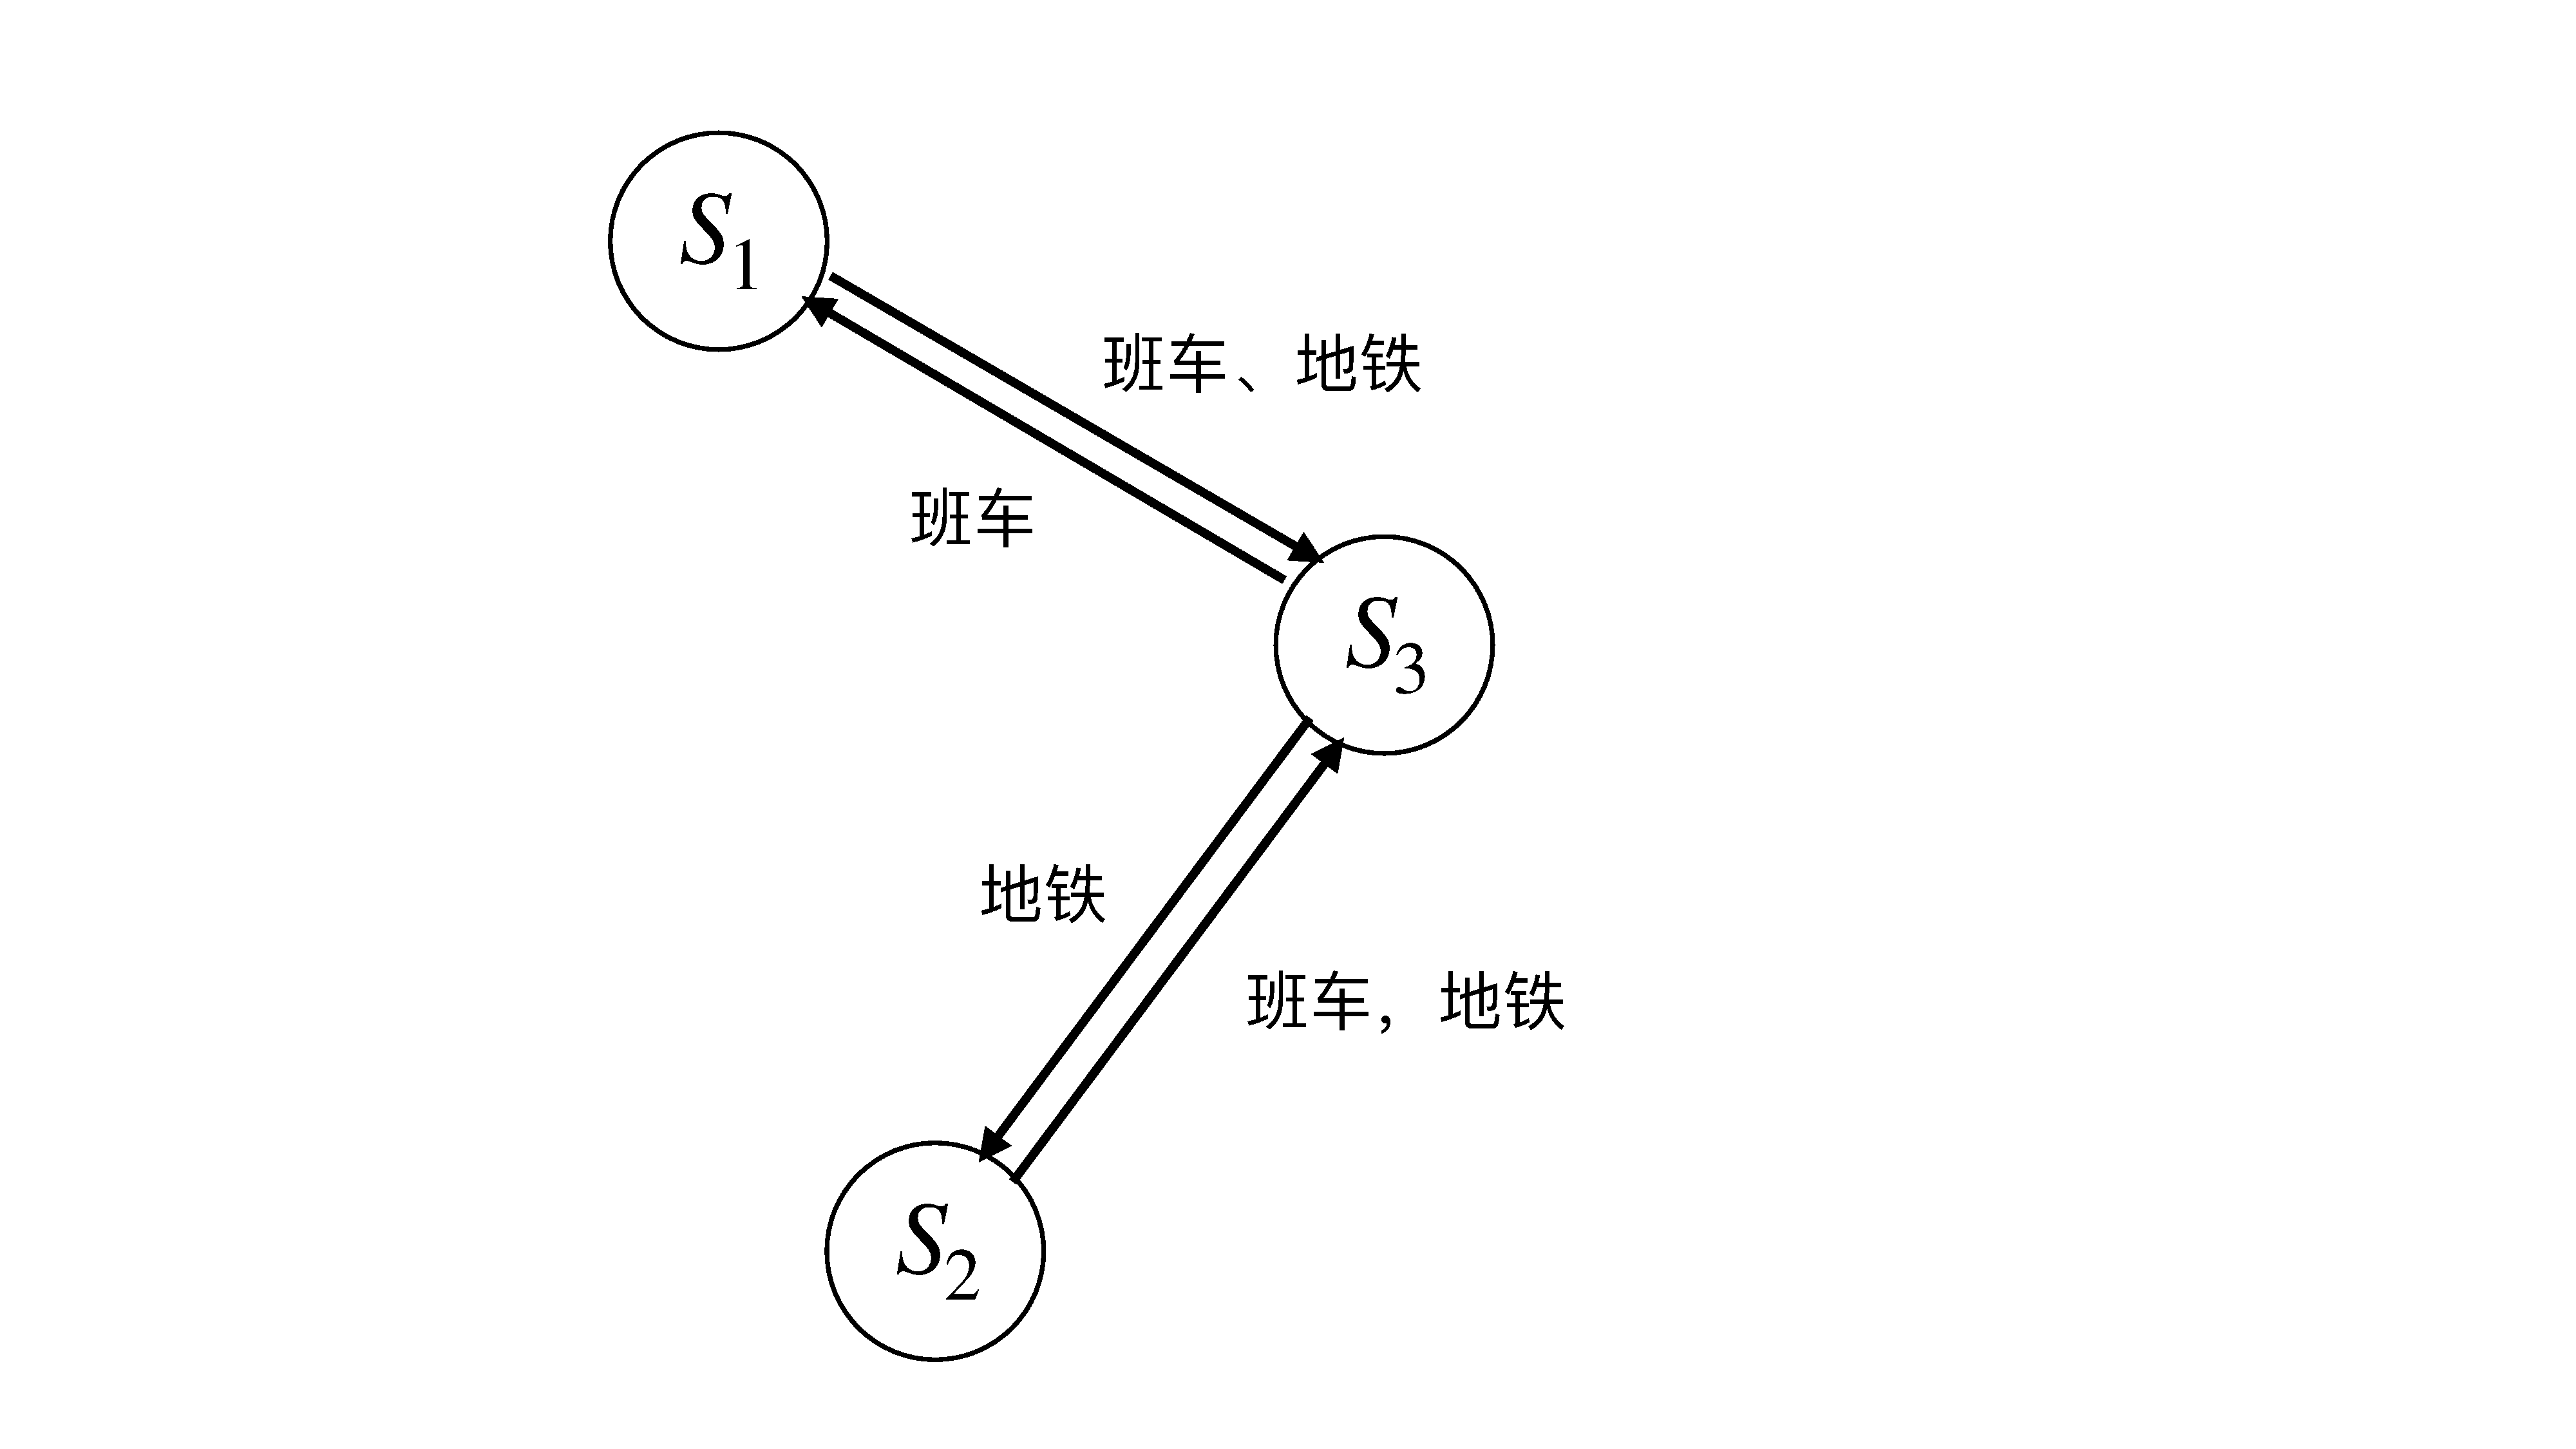
\includegraphics[width=0.5\linewidth]{Q1.pdf}
    \caption{研小理的通勤设计}
    \label{fig:Q1}
\end{figure}

\begin{enumerate}[label=(\roman*)]
\item 每个状态下可执行的动作:\textsc{班车}、\textsc{地铁}。  
所有转移与奖励都是确定性的。  
真实(但未知)的奖励如下表所示:

\begin{table}[h!]
\centering
\begin{tabular}{@{}lcc@{}}
\toprule
奖励 & 班车 & 地铁 \\ \midrule
$S_1$ & +0.7 & $-1.0$ \\
$S_2$ & +1.0 & $-1.3$ \\
$S_3$ & $-0.5$ & $-0.7$ \\ \bottomrule
\end{tabular}
\captionof{table}{通勤MDP的奖励函数}
\end{table}
折扣因子 $\gamma = 0.9$。运行值迭代后,你得到如下最优 $Q$-值:

\begin{table}[h!]
\centering
\begin{tabular}{@{}lcc@{}}
\toprule
$Q^*$ & 班车 & 地铁 \\ \midrule
$S_1$ & +1.65 & $-0.05$ \\
$S_2$ & +1.95 & $-0.35$ \\
$S_3$ & +0.98 & +1.05 \\ \bottomrule
\end{tabular}
\captionof{table}{最优三状态$Q$表}
\end{table}

\textbf{请问研小理通勤的最优策略是什么?[10分]}

\textbf{解答}:
\emph{请在此处填写解答。}
\vspace{1cm}


\item 现在考虑一种\emph{聚合}状态表示:将状态 $S_1$ 与 $S_2$ 合并成一个宏状态 $S_{12}$,而 $S_3$ 保持不变。你会发现可以直接用“在中关村”和“不在中关村”来代表这个MDP链,新的MDP只有两个状态:$S_{12}$ 和 $S_3$。  

在此聚合状态下(仍取 $\gamma = 0.9$),我们仍然在三状态环境中运行Q-learning,但是使用双状态的Q表,可以得到的$Q^*$值为

\begin{figure}[h!]
\centering
\begin{minipage}[b]{0.48\linewidth}
    \centering
    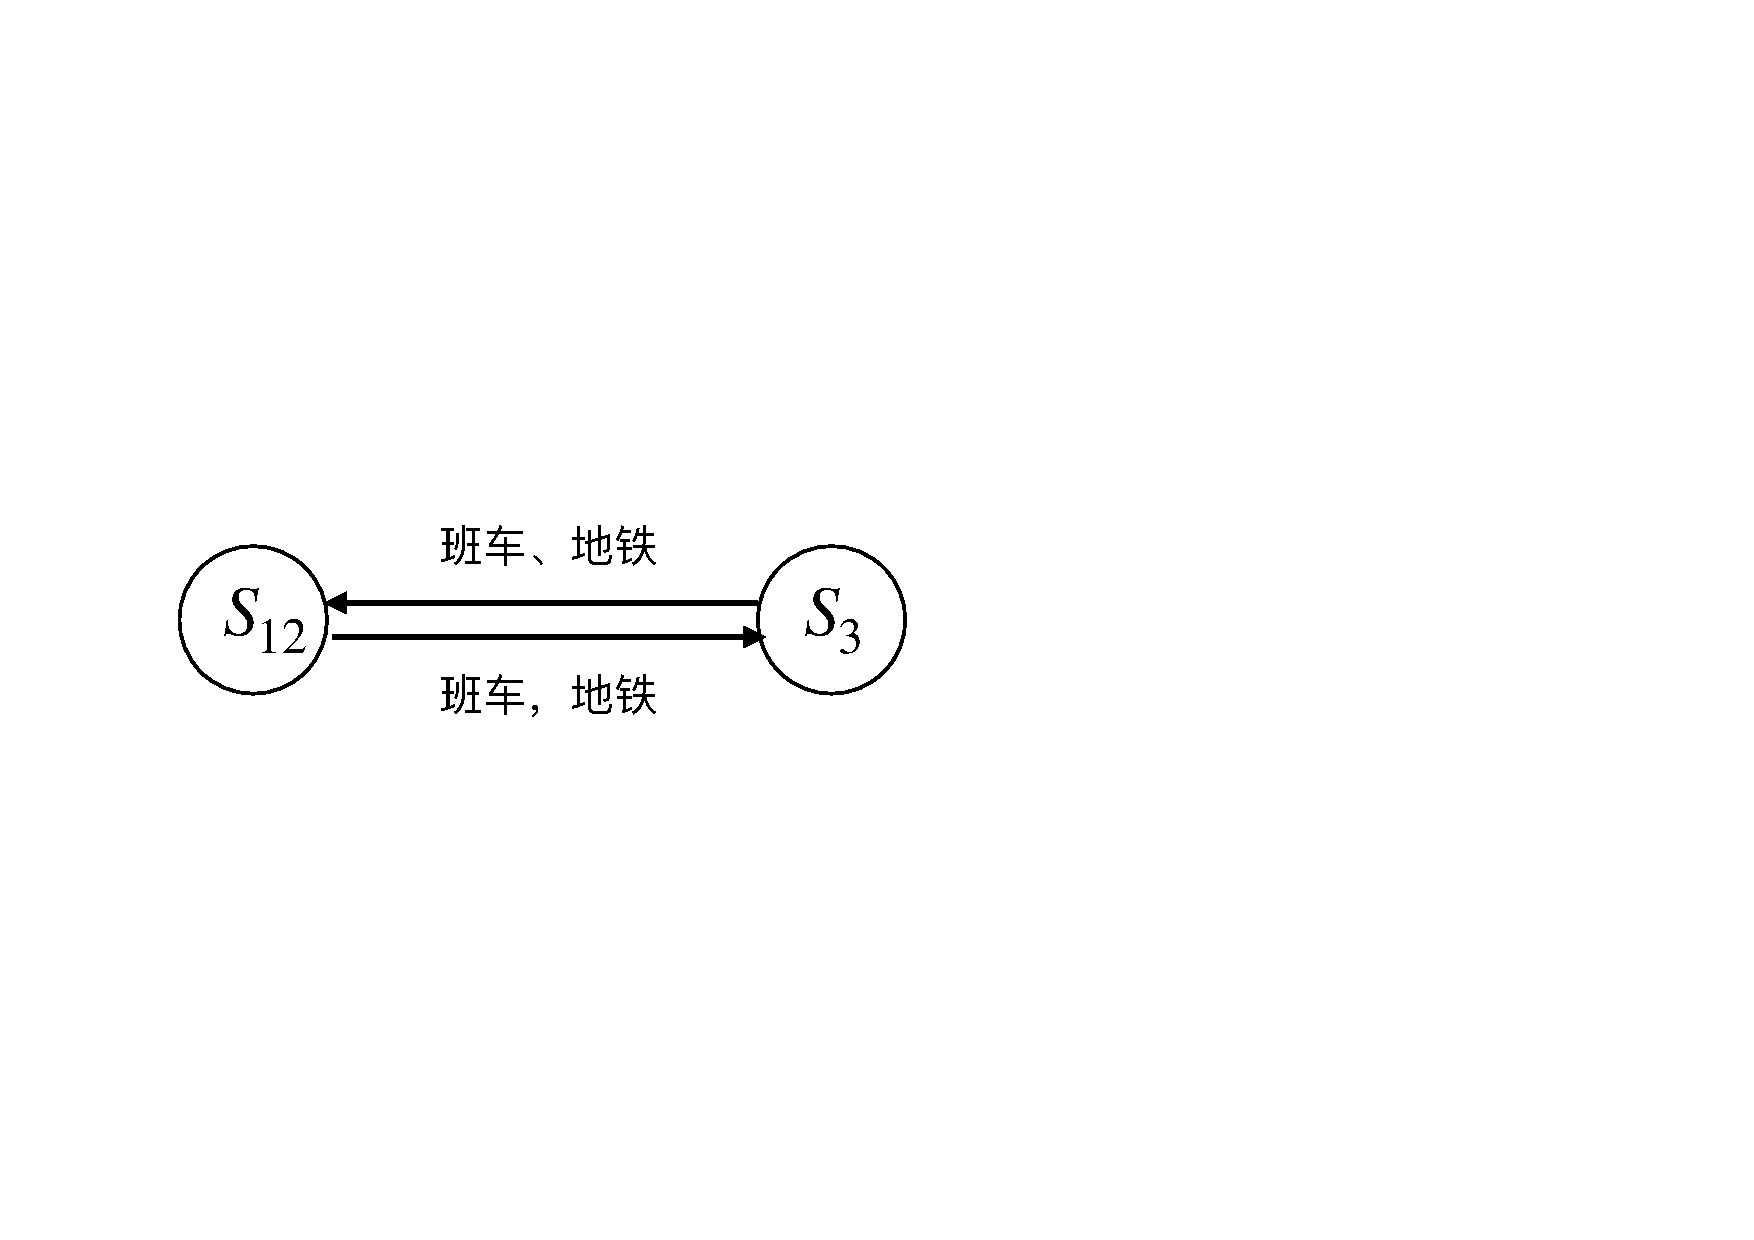
\includegraphics[width=\linewidth]{Q1_2.pdf}
    \caption{简化后的通勤MDP}
    \label{fig:Q1_2}
\end{minipage}
\hfill
\begin{minipage}[b]{0.45\linewidth}
    \centering
    \begin{tabular}{@{}lcc@{}}
        \toprule
        $Q^*$ & 班车 & 地铁 \\ \midrule
        $S_{12}$ & +1.73 & -0.08 \\
        $S_3$    & +1.03 & +0.84 \\ \bottomrule
    \end{tabular}
    \captionof{table}{两状态$Q^*$表}
    \label{tab:Q1}
\end{minipage}
\end{figure}

\textbf{根据这些 $Q$-值,最优策略是什么?与使用真实三状态表示时得到的最优策略相同?解释原因。 [30分]}  

\textbf{解答}:
    \emph{请在此处填写解答。}
    \vspace{1cm}


\end{enumerate}

\section{Frozenlake小游戏[60分,编程题]}

\subsection{简单介绍}

在本次编程作业中,将实现强化学习中的两种算法——策略迭代(Policy Iteration)和Q-Learning,并在Gymnasium(前身为OpenAI Gym)环境中的Frozenlake游戏环境中进行应用。通过这次作业,希望你可以理解这几种算法的工作原理及其在不同环境和奖励条件下的表现。非常鼓励探索和调整不同环境参数,分析算法在各种条件下的适应性和性能。

\begin{figure}[ht]
  \centering
    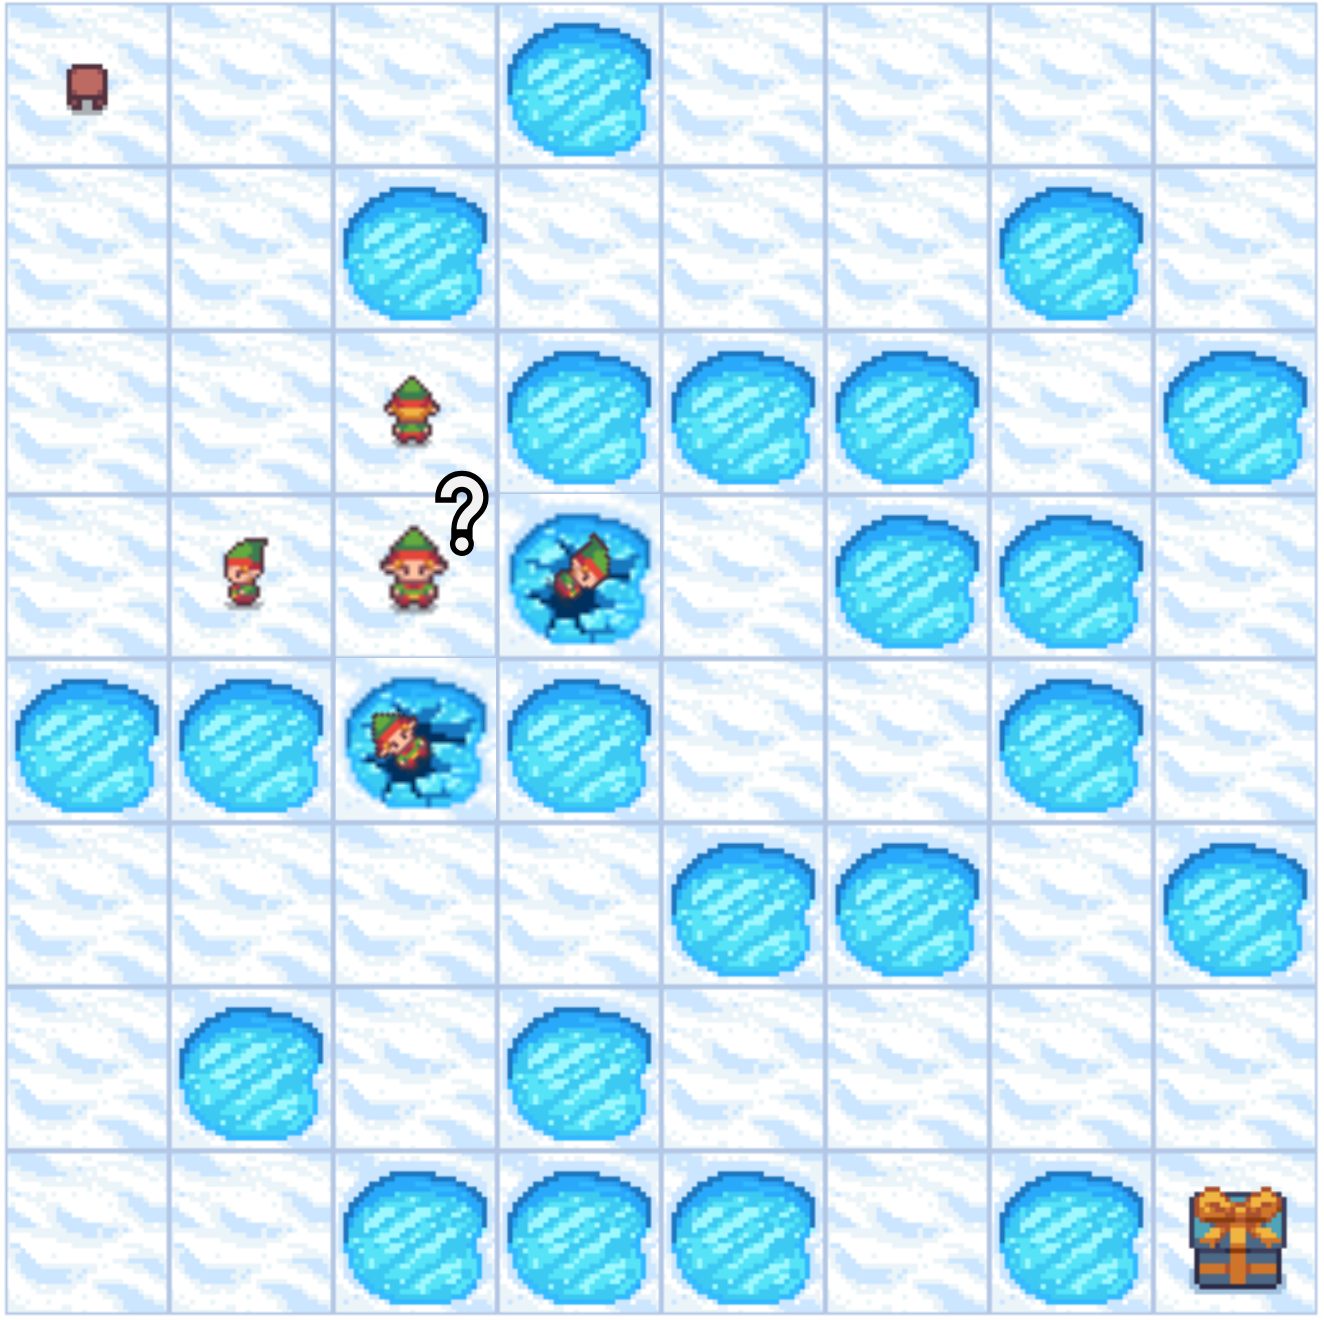
\includegraphics[width=0.5\textwidth]{frozenlake.png}
    \caption{Frozenlake小游戏画面(作业中不会出现此情况)}
  	\label{fig:frozenlake}
\end{figure}

\subsection{环境安装}

环境安装步骤:

\begin{enumerate}
    \item 确保你的系统已安装Python 3.9或更高版本。
    \item 创建并激活虚拟环境:
    \begin{minted}{bash}
    python -m venv frozenlake_env
    source frozenlake_env/bin/activate  % 在Linux或macOS上
    % 或
    frozenlake_env\Scripts\activate  % 在Windows上
    \end{minted}
    \item 安装所需的包:
    \begin{minted}{bash}
    pip install -r requirements.txt
    \end{minted}
\end{enumerate}

这样就完成了简单的环境配置,可以开始你的Frozenlake编程作业了。

\subsection{快速开始}

\begin{enumerate}
    \item 直接运行下面命令即可快速看到运行效果,注意此时你还没有实现任何算法,智能体的动作完全是从动作空间随机采样的:
    \begin{minted}{bash}
    python run.py
    \end{minted}
    \item 你可以通过修改 \mintinline{bash}{config.yaml} 文件来自定义参数。以下是一些可以调整的主要参数:
    \begin{itemize}
        \item 环境参数:
        \begin{itemize}
            \item \mintinline{python}{map_size}: 地图大小
            \item \mintinline{python}{frozen_prob}: 冰面出现的概率
            \item \mintinline{python}{is_slippery}: 是否设置冰面为滑动的
            \item \mintinline{python}{render_mode}: 渲染模式
        \end{itemize}
        \item policy\_iteration 的参数:
        \begin{itemize}
            \item \mintinline{python}{gamma}: 折扣因子
            \item \mintinline{python}{tol}: 收敛容差
        \end{itemize}
        \item qlearning 的参数:
        \begin{itemize}
            \item \mintinline{python}{num_episodes}: 训练回合数
            \item \mintinline{python}{gamma}: 折扣因子
            \item \mintinline{python}{learning_rate}: 学习率
            \item \mintinline{python}{epsilon}: 初始探索率
            \item \mintinline{python}{epsilon_decay}: 探索率衰减速度
        \end{itemize}
    \end{itemize}
    修改这些参数后,重新运行 \mintinline{bash}{python run.py} 即可看到不同设置下的算法表现。
    \item 如果你想快速运行多组实验进行算法效果对比,可以使用 \mintinline{bash}{--multirun} 参数:
    \begin{minted}{bash}
    python run.py --multirun \
        algorithm=policy_iteration,QLearning \
        env.is_slippery=False,True \
        env.render_mode=ansi
    \end{minted}
    这将同时运行4种组合的实验(上面命令在windows中最好写成一行执行):
    \begin{itemize}
        \item \mintinline{python}{policy_iteration} 算法在不滑动冰面和滑动冰面下的效果
        \item \mintinline{python}{QLearning} 算法在不滑动冰面和滑动冰面下的效果
    \end{itemize}
    你可以根据需要调整参数组合,以进行更多的对比实验。
\end{enumerate}

\subsection{题目要求}

\begin{enumerate}[label=(\roman*)]
\item 请实现策略迭代算法,并在确定性环境中运行,记录结果 [20分]。

\textbf{解答}:

    % Student mode content: answers are hidden
    \emph{请在此处粘贴代码。}
    \vspace{2cm}

\item 请实现Q-Learning算法,并在确定性环境中运行,记录结果 [20分]。

\textbf{解答}:

    \emph{请在此处粘贴代码。}
    \vspace{2cm}


\item 在随机性环境中,分别运行策略迭代和Q-Learning算法,比较两者的表现,并分析原因 [10分]。

可以使用以下代码来运行对比不同环境的算法表现:

\begin{minted}{bash}
python run.py --multirun \
    env.is_slippery=False,True \
    algorithm=policy_iteration,QLearning \
    env.render_mode=ansi
\end{minted}

\textbf{解答}:


    \emph{请在此处粘贴结果。}
    \vspace{1cm}


\item 上述三小问的地图长度为4,修改地图长度为\{6, 8\},再次运行策略迭代和Q-Learning算法,比较两者的表现,并分析原因 [10分]。

\textbf{解答}:


    \emph{请在此处粘贴结果。}
    \vspace{1cm}

\end{enumerate}
\begin{appendices}

\subsection*{requirements.txt}
\begin{minted}{text}
gymnasium[toy_text]
hydra-core
\end{minted}

\subsection*{run.py}
\begin{minted}{python}
"""
This script is the main entry point for the project. It uses Hydra to manage the 
configuration and runs the selected algorithm on the FrozenLake environment.

This file does not need to be modified. The algorithms that need to be modified 
are in the algorithm.py files.
"""

import gymnasium
import hydra
import numpy as np
from gymnasium.envs.toy_text.frozen_lake import FrozenLakeEnv, generate_random_map
from algorithm import PType, policy_iteration, QLearning
from config import Config
from typing import Callable

def render_result(
    env: gymnasium.Env, 
    policy: np.ndarray = None, 
    max_steps: int = 100,
    test_iter: int = 100,
):
    """
    This function does not need to be modified
    Renders policy once on environment. Watch your agent play!

    Parameters
    ----------
    env: gymnasium.Env
        Environment to play on. Must have nS, nA, and P as
        attributes.
    Policy: np.array of shape [nS] or [nS x nA]
        The action to take at a given state or the state-action values.
    """
    episode_reward = 0
    average_steps = 0
    for iter in range(test_iter):
        state, info = env.reset()
        for t in range(max_steps):
            if policy is None:
                action = env.action_space.sample()
            else:
                if policy.ndim == 2:
                    action = np.argmax(policy[state])
                else:
                    action = policy[state]
            state, reward, done, _, _ = env.step(action)
            # if reward == 0:
            #     reward = 2
            episode_reward += reward
            if done:
                average_steps += t
                break
        if not done:
            print(f"The agent didn't reach a terminal state in {max_steps} steps.")
    print("Episode reward: %f" % episode_reward)
    print("Average number of steps: %f" % (average_steps / test_iter))

def get_method(algorithm: str) -> Callable:
    if algorithm == "policy_iteration":
        return policy_iteration
    elif algorithm == "QLearning":
        return QLearning
    else:
        return None

@hydra.main(config_path=".", config_name="config.yaml", version_base=None)
def main(cfg: Config) -> None:
    # from omegaconf import DictConfig, OmegaConf
    # print(OmegaConf.to_yaml(cfg))
    # return    
    env = FrozenLakeEnv(
        desc = generate_random_map(
            size = cfg.env.map_size, 
            p = cfg.env.frozen_prob,
            seed = cfg.env.seed
        ),
        is_slippery = cfg.env.is_slippery,
        render_mode = cfg.env.render_mode
    )

    P: PType = env.P
    nS:int = env.observation_space.n
    nA:int = env.action_space.n

    gamma:float = cfg.policy_iteration.gamma
    tol:float = cfg.policy_iteration.tol

    num_episodes = cfg.qlearning.num_episodes
    gamma = cfg.qlearning.gamma
    learning_rate = cfg.qlearning.learning_rate
    epsilon = cfg.qlearning.epsilon
    epsilon_decay = cfg.qlearning.epsilon_decay
    if cfg.env.render_mode == 'human':
        test_iter = 1
    else:
        test_iter = 100

    def _play(method: Callable):
        if method is None:
            print(f"\n{'-' * 27}\nBeginning RANDOM_SAMPLE\n{'-' * 27}")
            render_result(env, max_steps=cfg.render.max_steps)
            return

        print(f"\n{'-' * 27}\nBeginning {method.__name__.upper()}\n{'-' * 27}")
        if method.__name__ == "QLearning":
            env.render_mode = 'ansi'
            # during training, we don't want to render the environment
            Q = method(
                env, 
                num_episodes, 
                gamma, 
                learning_rate, 
                epsilon, 
                epsilon_decay
            )
            env.render_mode = cfg.env.render_mode
            render_result(env, Q, cfg.render.max_steps, test_iter)
        elif method.__name__ == "policy_iteration":
            V, p = method(P, nS, nA, gamma, tol)
            render_result(env, p, cfg.render.max_steps, test_iter)
        else:
            raise ValueError(f"Method {method.__name__} not recognized.")
    
    _play(get_method(cfg.algorithm))
    env.close()

if __name__ == "__main__":
    main()
    
# python run.py
\end{minted}

\subsection*{config.yaml}
\begin{minted}{yaml}
env:
  map_size: 4  # Size of the environment map
  frozen_prob: 0.8  # Probability of frozen tiles appearing
  seed: 20241022  # Random seed for map generation
  is_slippery: False  # Whether to set the ice surface as slippery
  render_mode: human  # Render mode: human (visual) or ansi (text mode)
policy_iteration:
  gamma: 0.9  # Discount factor for future rewards
  tol: 1e-3  # Convergence tolerance for determining algorithm termination
qlearning:
  num_episodes: 2000  # Total number of training episodes
  gamma: 0.9  # Discount factor for future rewards
  learning_rate: 0.1  # Learning rate
  epsilon: 0.8  # Initial exploration rate for ε-greedy strategy
  epsilon_decay: 0.99  # Decay rate of exploration rate
render:
  max_steps: 100  # Maximum number of steps per episode
algorithm: None  # Algorithm to use: policy_iteration, QLearning
\end{minted}

\subsection*{config.py}
\begin{minted}{python}
from dataclasses import dataclass
from omegaconf import MISSING

@dataclass
class EnvConfig:
    map_size: int = MISSING
    frozen_prob: float = MISSING
    seed: int = MISSING
    is_slippery: bool = MISSING
    render_mode: str = MISSING

@dataclass
class PolicyIterationConfig:
    gamma: float = MISSING
    tol: float = MISSING

@dataclass
class QLearningConfig:
    num_episodes: int = MISSING
    gamma: float = MISSING
    learning_rate: float = MISSING
    epsilon: float = MISSING
    epsilon_decay: float = MISSING

@dataclass
class RenderConfig:
    max_steps: int = MISSING

@dataclass
class Config:
    env: EnvConfig = MISSING
    policy_iteration: PolicyIterationConfig = MISSING
    qlearning: QLearningConfig = MISSING
    render: RenderConfig = MISSING
    algorithm: str = MISSING
\end{minted}

\subsection*{algorithm.py}
\begin{minted}{python}
"""
In this file, you will implement Policy Iterations and 
Q-learning algorithms.
"""

"""
------Below is the implementation of Policy Iteration------
You will implement policy iteration first.

For policy_evaluation, policy_improvement, policy_iteration 
and value_iteration, the parameters `P, nS, nA, gamma` are 
defined as follows:

- P: `Dict[int, Dict[int, List[Tuple[float, int, int, bool]]]]`
    For each pair of states in [1, nS] and actions in [1, nA],
    `P[state][action]` is a tuple of the form `(probability, 
    nextstate, reward, terminal)` where
        - `probability`: `float`
            the probability of transitioning from "state" to 
            "nextstate" with "action"
        - `nextstate`: `int`
            denotes the state we transition to (in range [0, 
            nS - 1])
        - `reward`: `int`
            either 0 or 1, the reward for transitioning from 
            "state" to "nextstate" with "action"
        - `terminal`: `bool`
            True when "nextstate" is a terminal state (hole or 
            goal), False otherwise
- `nS`: `int`
    number of states in the environment
- `nA`: `int`
    number of actions in the environment
- `gamma`: `float`
    Discount factor. Number in range [0, 1)
"""

import numpy as np
from typing import Dict, List, Tuple

__all__ = [
    "PType",
    "policy_iteration", 
    "QLearning"
]

PType = Dict[
    int, 
    Dict[
        int, 
        List[
            Tuple[
                float, 
                int, 
                int, 
                bool
            ]
        ]
    ]
]

def policy_evaluation(
    P: PType, 
    nS: int, 
    nA: int, 
    policy: np.ndarray, 
    gamma: float = 0.9, 
    tol: float = 1e-3
) -> np.ndarray:
    """Evaluate the value function from a given policy.

    Parameters
    ----------
    P, nS, nA, gamma:
            defined at beginning of file
    policy: np.array[nS]
            The policy to evaluate. Maps states to actions.
    tol: float
            Terminate policy evaluation when
        max |value_function(s) - prev_value_function(s)| < tol
    
    Returns
    -------
    value_function: np.ndarray[nS]
            The value function of the given policy, where 
            value_function[s] is the value of state s
    """

    value_function = np.zeros(nS)
    ############################
    # YOUR IMPLEMENTATION HERE #
    ############################
    return value_function


def policy_improvement(
    P: PType,
    nS: int,
    nA: int,
    value_from_policy: np.ndarray,
    policy: np.ndarray,
    gamma: float = 0.9
) -> np.ndarray:
    """Given the value function from policy improve the policy.

    Parameters
    ----------
    
    P, nS, nA, gamma:
            defined at beginning of file
    value_from_policy: np.ndarray
            The value calculated from the policy
    policy: np.array
            The previous policy.

    Returns
    -------
    new_policy: np.ndarray[nS]
            An array of integers. Each integer is the optimal 
            action to take in that state according to the 
            environment dynamics and the given value function.
    """

    new_policy = np.zeros(nS, dtype="int")
    ############################
    # YOUR IMPLEMENTATION HERE #
    ############################
    return new_policy


def policy_iteration(
    P: PType, 
    nS: int, 
    nA: int, 
    gamma: float = 0.9, 
    tol: float = 1e-3
) -> Tuple[np.ndarray, np.ndarray]:
    """Runs policy iteration.

    You should call the policy_evaluation() and 
    policy_improvement() methods to implement this method.

    Parameters
    ----------
    P, nS, nA, gamma:
            defined at beginning of file
    tol: float
            tol parameter used in policy_evaluation()
    

    Returns
    ----------
    value_function: np.ndarray[nS]
            The final value function of the policy after 
            convergence
    policy: np.ndarray[nS]
            The final policy after convergence
    """

    value_function = np.zeros(nS)
    policy = np.zeros(nS, dtype=int)

    ############################
    # YOUR IMPLEMENTATION HERE #
    ############################
    return value_function, policy


"""
------Below is the implementation of QLearning------

For the QLearning and SARSA functions, the parameters `env, 
num_episodes, gamma, lr, epsilon, epsilon_decay` are defined 
as follows:

- `env`: `gymnasium.Env`
    The environment used to compute the Q function. Must have 
    observation_space and action_space attributes.
- `num_episodes`: `int`
    Number of training episodes.
- `gamma`: `float`
    Discount factor. Value in range [0, 1)
- `lr`: `float`
    Learning rate. Value in range [0, 1)
- `epsilon`: `float`
    Epsilon value used in the ε-greedy method.
- `epsilon_decay`: `float`
    Rate at which epsilon decreases. Value in range [0, 1)

Both functions return a numpy array of shape [nS x nA], 
representing state-action values.
"""
import gymnasium

def QLearning(
    env:gymnasium.Env, 
    num_episodes=2000, 
    gamma=0.9, 
    lr=0.1, 
    epsilon=0.8, 
    epsilon_decay=0.99
) -> np.ndarray:
    """Learn state-action values using the Q-learning 
    algorithm with epsilon-greedy exploration strategy.
    Update Q at the end of every episode.

    Parameters
    ----------
    env: gymnasium.Env
        Environment to compute Q function for. Must have nS, 
        nA, and P as
    attributes.
    num_episodes: int
        Number of episodes of training.
    gamma: float
        Discount factor. Number in range [0, 1)
    learning_rate: float
        Learning rate. Number in range [0, 1)
    epsilon: float
        Epsilon value used in the epsilon-greedy method.
    epsilon_decay: float
        Rate at which epsilon falls. Number in range [0, 1)

    Returns
    -------
    np.array
        An array of shape [nS x nA] representing state, action 
        values
    """

    nS:int = env.observation_space.n
    nA:int = env.action_space.n
    Q = np.zeros((nS, nA))
    ############################
    # YOUR IMPLEMENTATION HERE #
    ############################
    return Q

\end{minted}

\end{appendices}
\end{document}
